% Template for Cogsci submission with R Markdown

% Stuff changed from original Markdown PLOS Template
\documentclass[10pt, letterpaper]{article}

\usepackage{cogsci}
\usepackage{pslatex}
\usepackage{float}
\usepackage{caption}

% amsmath package, useful for mathematical formulas
\usepackage{amsmath}

% amssymb package, useful for mathematical symbols
\usepackage{amssymb}

% hyperref package, useful for hyperlinks
\usepackage{hyperref}

% graphicx package, useful for including eps and pdf graphics
% include graphics with the command \includegraphics
\usepackage{graphicx}

% Sweave(-like)
\usepackage{fancyvrb}
\DefineVerbatimEnvironment{Sinput}{Verbatim}{fontshape=sl}
\DefineVerbatimEnvironment{Soutput}{Verbatim}{}
\DefineVerbatimEnvironment{Scode}{Verbatim}{fontshape=sl}
\newenvironment{Schunk}{}{}
\DefineVerbatimEnvironment{Code}{Verbatim}{}
\DefineVerbatimEnvironment{CodeInput}{Verbatim}{fontshape=sl}
\DefineVerbatimEnvironment{CodeOutput}{Verbatim}{}
\newenvironment{CodeChunk}{}{}

% cite package, to clean up citations in the main text. Do not remove.
\usepackage{apacite}

% KM added 1/4/18 to allow control of blind submission
\cogscifinalcopy

\usepackage{color}

% Use doublespacing - comment out for single spacing
%\usepackage{setspace}
%\doublespacing


% % Text layout
% \topmargin 0.0cm
% \oddsidemargin 0.5cm
% \evensidemargin 0.5cm
% \textwidth 16cm
% \textheight 21cm

\title{English Negative Constructions and Communicative Functions in Child
Language}


\author{{\large \bf Zoey Liu (ying.liu.5@bc.edu)} \\ Department of Computer Science \\ Boston College \AND {\large \bf Masoud Jasbi (jasbi@ucdavis.edu)} \\ Department of Linguistics \\ University of California, Davis}


\begin{document}

\maketitle

\begin{abstract}
How does negation develop in early child language? Previous research has
hypothesized that negation develops to serve specific communicative
functions such as rejection, prohibition, or non-existence, and that
different functions of negation are developed in distinct stages.
However, the evidence for such stages is mixed, leaving the possibility
that the multiple functions of negation have similar developmental paths
since the beginning. Leveraging automatic annotations of large-scale
child speech corpora in English, we examine the production trajectores
of seven negative constructions that tend to convey communicative
functions previously discussed in the literature. The results
demonstrate the emergence and gradual increase of these constructions in
child speech within the age range of 18-36 months. Production mostly
remains stable, regular, and close to parents' levels after this age
range. These findings are consistent with negation starting as an
abstract multi-functional concept. Alternatively, it is possible that
the developmental stages of different negative constructions happen
relatively quickly within 18-36 months and therefore their orders of
development could not be detected in children's production using our
methods.

\textbf{Keywords:}
negation; syntactic construction; communicative function; development;
child language.
\end{abstract}

\hypertarget{introduction}{%
\section{Introduction}\label{introduction}}

Negation is an abstract concept crucial to everyday communication. It
could be used in a sign like ``no mask, no entry'' to regulate people's
behaviors; an employee could say ``I don't like Mondays'' to communicate
their desires or dislikes. But how does the multi-functional concept of
negation emerge and develop in the human mind? Are early developmental
stages of negation restricted to just a few communicative functions in
child language? Or do negative utterances that play different functions
share common developmental paths from the start?

Around a century and a half ago, Darwin (1872) thought that negation
developed from the expression of human emotions and desires. He
hypothesized the earliest manifestation of negation in infants is when
they refuse food from parents by withdrawing their heads laterally
(within specific cultural traditions). Similarly, many researchers
studying early functions of negative morphemes like \emph{no} proposed
that children use negation to ``reject'' or ``refuse'' (Bloom, 1970).
For example, when they are asked ``do you want juice?'', they may say
``no'', ``not want it'', or ``don't like it''. Pea (1978) proposed
``rejection'' as the first function of negation in child language.

Bloom (1970) argued that the use of negation to express
``non-existence'' emerges before ``rejection''. For example, when an
object that children expect to be present is not, children may say:
``there is no window''. Two close concepts to non-existence discussed in
the literature are ``disappearance'' and ``non-occurrence'' (Pea, 1978;
Villiers \& Villiers, 1979). Disappearance refers to situations where an
object disappears and children use negation to describe it (e.g.~``no
more noise''). Non-occurrence refers to cases when an expected action or
event does not occur, as in ``not working'' or ``doggie not barking''
(Cameron-Faulkner, Lieven, \& Theakston, 2007; Choi, 1988).
Additionally, non-existence could also be expressed by combining
negation with locative prepositional phrases (e.g.~``no in there'').
While rejection was hypothesized to interact with human emotions and
desires, non-existence (broadly construed to include ``disappearance''
and ``non-occurrence'') likely interacts with perception.

Choi (1988) argued that the ``prohibition'' function of negation emerges
as early as rejection and non-existence. In cases of prohibition,
children use negation to stop others or themselves from performing
actions (e.g.~``don't go''). A function similar to prohibition is
``inability'' (e.g.~``I cannot zip it''), in that both involve
conceptualizing actions and negating them. Choi (1988) suggested that
expressions of inability emerge after the functions in the first phase,
namely non-existence, rejection, and prohibition.

Bloom (1970) defined the function of ``denial'' for negation as
asserting that ``an actual or supposed predication was not the case''.
Later researchers formulated it as ``truth-functional negation'' because
it is used to negate the truth of a proposition (Cameron-Faulkner et
al., 2007; Pea, 1978). A particular sub-function of denial is
``labeling'', which is realized as the negation of a nominal or
adjectival predicate such as ``this is not a bunny'' or ``not red''.
These utterances are often used to introduce new linguistic labels by
parents and in turn might facilitate word learning (Clark, 2010).

Despite considerable research on early functions of negation, their
developmental trajectories in children's production have remained
unclear. Prior work has claimed different orders of development (Pea,
1978). Recently, Nordmeyer \& Frank (2018) looked at the speech of five
children in the Providence corpus (Demuth, Culbertson, \& Alter, 2006)
and found a great deal of individual variation in how early a negative
function is attested. They reported that their findings are not as
consistent as previously claimed. This leaves the possibility that
across (a larger number of) children, distinct functions of negation
could develop within the same age range and have similar production
trajectories.

In order to assess this possibility, we need to study much larger amount
of child production data and more children than before. Previous
experiments have mainly relied on manual annotations of corpus data to
determine the communicative function of a given negative utterance,
which in turn has limited their work to only a handful of children per
study.

Here we aim to go beyond existing work via utilizing a large collection
of child speech corpora in English (MacWhinney, 2000) along with
computational tools to automatically identify negative utterances that
tend to convey the communicative functions discussed in prior research
(Table 1). In particular, our study investigates three questions: (1)
how does the developmental trajectory of the negative constructions for
each function look like? (2) for utterances expressing the same
function, does the developmental trajectory differ depending on
particular lexical items that negation modifies (e.g.~\emph{like} or
\emph{want} for rejection)? (3) taking all functions into account, do
they share similar developmental characteristics, or would there be
function-specific differences?

Given the automatic fashion of our approach, we focus on larger/longer
negative constructions at the single-sentence level such as ``I don't
like that'' or ``I can't jump''. This is in opposition to short negative
forms at the discourse-level such as cases consisting of one
(e.g.~``no!'') or repetition of negative morphemes (e.g.~``no no no'').
These shorter negative utterances arguably could express multiple
functions when not taking the discourse context into account and
accordingly leave more room for ambiguous interpretation. Therefore the
negative utterances understudied in our experiments do not fully cover
all negation instances from the corpora investigated, nor reflect all
possible communicative functions that could be played by negation more
broadly, but it could provide at least a conservative estimate of the
age range during which negation is developed gradually in child
production.

\begin{table*}[h]
\small
\centering
\begin{tabular}{rrr}
  \hline
 \textbf{Function} & \textbf{Linguistic Composition} & \textbf{Examples} \\
  \hline
Rejection & with \textit{like} or \textit{want} & \textit{I not like it}, \textit{not want it}  \\
Non-existence & expletives & \textit{there is no soup} \\
Prohibition & with imperative subjectless \textit{do} & \textit{do not spill milk} \\
Inability & with modal \textit{can} & \textit{I cannot zip it} \\
Labeling & modifying nominal or adjectival predicatives & \textit{that's not a crocodile}; \textit{it's no interesting} \\
Epistemic negation & with \textit{know}, \textit{think}, \textit{remember}  & \textit{I not know} \\
Possession & with \textit{have}; or possesive pronouns & \textit{not have the toy}; \textit{not mine} \\
   \hline
\end{tabular}
\caption{Communicative functions of negation in early child language of English.}
\end{table*}

\hypertarget{experiments}{%
\section{Experiments}\label{experiments}}

\hypertarget{data-and-preprocessing}{%
\subsection{Data and preprocessing}\label{data-and-preprocessing}}

For developmental production data of child language in English, we
turned to the CHILDES database (MacWhinney,
2000).\footnote{Code and data are in quarantine at \url{https://github.com/zoeyliu18/Negative_Constructions.}}.
We focused on speech produced by children with typical development
within the age range of 12 - 72 months. Utterances of child and parent
speech were extracted via the childes-db (Sanchez et al., 2019)
interface using the programming language R. Negative structures were
then identified based on whether a structure contains any of the three
negative morphemes: \emph{no}, \emph{not} and \emph{n't}.

In order to conduct analysis of negative syntactic constructions and the
particular communicative functions that they serve, we need to first
obtain (morpho)syntactic representations of child and parent speech. To
do that, we opted for the dependency grammar framework (Tesnière, 1959);
the syntactic dependency relations of all negative utterances were
automatically derived with DiaParser (Attardi, Sartiano, \& Yu, n.d.), a
dependency parsing system that has been demonstrated to achieve
excellent performance for English. And to further facilitate
identifications of negative constructions, we also utilized the
available part-of-speech (POS) information initially provided by CHILDES
(Sagae, Davis, Lavie, MacWhinney, \& Wintner, 2010) when necessary.

Besides the functions of rejection, non-existence, prohibition,
inability and labeling (the sub-function of denial), we expanded with
two other functions: epistemic negation (Choi, 1988) and possession (see
Table 1). For each function, using our parsed data set, we characterized
the syntactic features of the negative constructions associated with
that function. Based on these features, negative utterances were
automatically extracted in a rule-based fashion with the help of POS
information and syntactic dependencies.

\hypertarget{measures}{%
\subsection{Measures}\label{measures}}

As indexes of the developmental trajectory for negative constructions
and their communicative functions in child speech, we measured the
following two metrics at each given age of the children. The first one
is the \emph{ratio} of negative utterances. For instance, the number of
utterances produced by children at the age of 30 months (not just all
negative constructions at this age) is 52,491 in total. Among these
utterances, negative structures that have the function of inability
occur for 141 times; the ratio for this communicative function at 30
months is then calculated as 141 / 52,491 = 0.003.

Given the noisy nature of child production data in general, and the
facts that there are different numbers of utterances and children at
each age, another measure that we utilized is \emph{moving ratio},
borrowed from the model of moving average in analyses of time series
data (Wei, 2006). For a communicative function, the goal of the moving
ratio is still to reflect the production of the negative utterances at
the given age; meanwhile it takes into account the previous production
of all negative constructions of the same function before the specified
age. This would allow us to have a more balanced look at individual
developmental stage (e.g.~age) of a communicative function, in relation
to its development patterns thus far.

The computation of the moving ratio is as follows. For instance, given
that the number of negative utterances that express inability in child
speech is 141 at the age of 30 months, we: (1) count the total number of
negative constructions with the same function produced by children
\emph{at and before} 30 months old (682); (2) compute the total number
of utterances (419,949) within the same age range; (3) divide the number
of (1) by that of (2) (682 / 419,949 = 0.002).

While our focus is negative utterances in child production, we used
parents' speech as comparative references. Therefore for every
communicative function, the same two ratio measures were calculated for
parent speech in a similar fashion. Our plots accordingly contrast the
ratio / moving ratio of different negative constructions between
children's and parents' production at corresponding ages of the
children.

In what follows, we describe in detail the results of each communicative
function and their negative constructions. While we computed both ratio
and moving ratio for every function, our analyses mainly rely on the
latter.

\hypertarget{communicative-functions-of-negative-constructions}{%
\subsection{Communicative functions of negative
constructions}\label{communicative-functions-of-negative-constructions}}

\hypertarget{rejection}{%
\subsubsection{Rejection}\label{rejection}}

For the function of rejection, we examined cases where the lemma of the
head verb of the phrase is either \emph{like} or \emph{want}, and the
head verb is modified by one of the three negative morphemes. Each of
the utterances either takes a subject or has no subject at all. And the
existence of a subject was determined via searching for a word in the
utterance that has the \emph{nsubj} dependency relation with the head
verb.

Additionally, other than expressions that the speakers used to describe
their own emotion, with (e.g.~(1)) or without (e.g.~(2)) an auxiliary
verb, we also included cases that express rhetorical inquiries of
emotions from one interlocutor addressed to another (e.g.~(3)) as well
as instances where the speaker is describing the emotion of somebody
else (e.g.~(4)). Overall our data extraction resulted in a total of
17,436 negative utterances (child: 7,395; parent: 10,041).

~ (1) \emph{I no like sea}

~ (2) \emph{don't wanna go}

~ (3) \emph{don't you wanna try it}

~ (4) \emph{Sarah doesn't like that either}

\begin{figure*}[h]

\begin{CodeChunk}


\begin{center}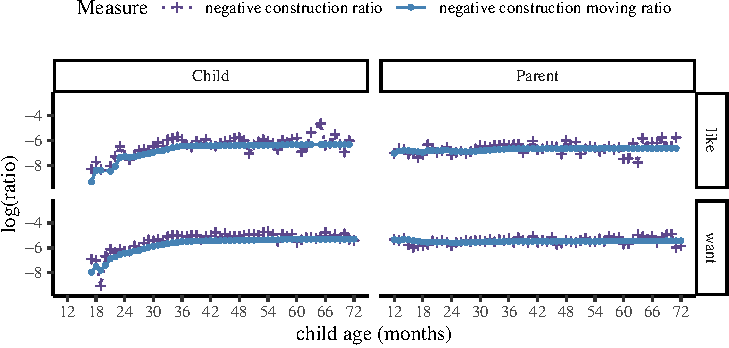
\includegraphics{figs/emotion-1} \end{center}

\end{CodeChunk}
\caption[This image spans both columns]{Rejection.}\label{fig:rejection}
\end{figure*}

As presented in Figure 1, within the context of the corpus data that we
analyzed, the overall pattern for children's usage of negative morphemes
for rejection is comparable regardless of the particular head verb.
Comparing child and parent speech, it seems that children's production
of rejection is gradually increasing between the age of 18 to 36 months.
And the production moving ratio in child speech appears to be more
comparable to that of parent speech after 32-34 months.

\hypertarget{non-existence}{%
\subsubsection{Non-existence}\label{non-existence}}

For the function of non-existence, in order to not confuse with the
function of labeling (see below), we extracted utterances that have
expletives marked by \emph{there} (e.g.~(5) and (6)), and that the
predicate modified by the negative morphemes is a nominal phrase (headed
by either nouns or pronouns). This led to a total of 1,611 negative
utterances (child: 406; parent: 1,205).

~ (5) \emph{there's no (more) water}

~ (6) \emph{there isn't it}

In child speech, the production of negative constructions to express
non-existence is gradually increasing from 25 to 36 months (Figure 2),
which is by contrast later than that for the communicative function of
rejection presented in Figure 1. This is observation does not seem to
align with Bloom (1970), which initially proposed that the development
of non-existence is earlier than that of rejection. On the other hand,
children's production moving ratio gradually approaches that in parent
speech at 36-38 months.

Notice that there appears to be fluctuations of moving ratios between
the age of 19 and 25 months regarding child production. A closer
inspection of the data reveals that within that age range, the frequency
of negative utterances at most ages is either one or zero. Therefore
while the number of total utterances increases along the developmental
trajectory, the moving ratio for negative utterances actually decreases.

\begin{figure*}[h]

\begin{CodeChunk}


\begin{center}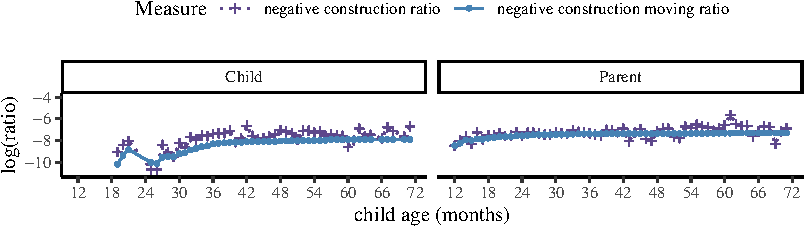
\includegraphics{figs/existence-1} \end{center}

\end{CodeChunk}
\caption[This image spans both columns]{Non-existence.}\label{fig:non-existence}
\end{figure*}

\hypertarget{prohibition}{%
\subsubsection{Prohibition}\label{prohibition}}

For constructions that articulate the function of prohibition, we
focused on cases that are annotated as imperatives from the initial
CHILDES annotations. These utterances do not take any subject; the
negative morphemes are combined with the auxiliary verb \emph{do}
(\emph{do}, \emph{does}, \emph{did}) and they together modify the head
verbs of the sentences. In order to not overlap with rejection,
non-existence, epistemic negation and possession (see below), our search
excluded cases where the head verb has any of the following lemma forms:
\emph{like}, \emph{want}, \emph{know}, \emph{think}, \emph{remember},
\emph{have}. This resulted in a total of 938 negative utterances (child:
267; parent: 671).

Based on Figure 3, children are combining negative morphemes for
prohibition more and more regularly amid 24-36 months, which is
comparable to that of the function of non-existence, but later than that
of rejection. This finding contrasts the proposal from Choi (1988),
which suggested that the development of these three functions
\emph{starts} around similar time. In comparison, the production moving
ratio in child speech for prohibition is consistently lower than that in
parent speech at any age of the children.

~ (7) \emph{don't blame Charlotte}

\begin{figure*}[h]

\begin{CodeChunk}


\begin{center}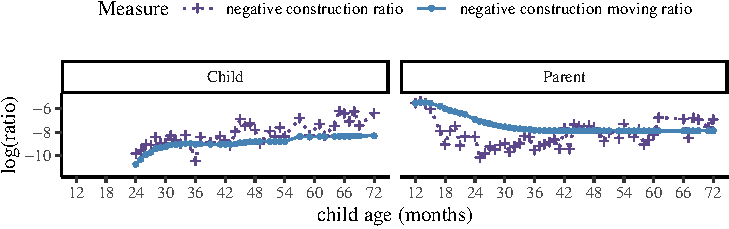
\includegraphics{figs/prohibition-1} \end{center}

\end{CodeChunk}
\caption[This image spans both columns]{Prohibition.}\label{fig:prohibition}
\end{figure*}

\begin{figure*}[h]

\begin{CodeChunk}


\begin{center}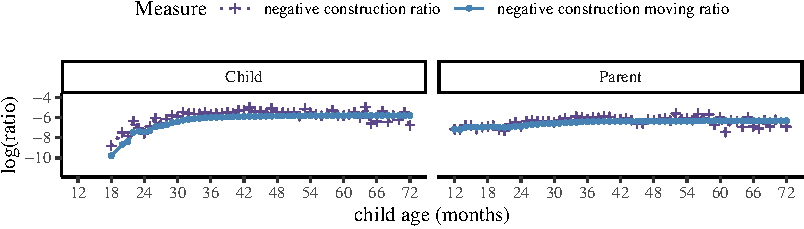
\includegraphics{figs/inability-1} \end{center}

\end{CodeChunk}
\caption[This image spans both columns]{Inability.}\label{fig:inability}
\end{figure*}

\begin{figure*}[h!]

\begin{CodeChunk}


\begin{center}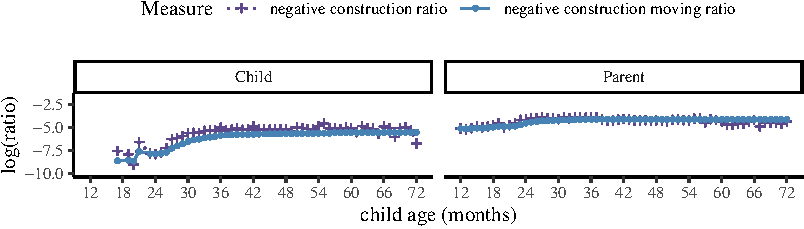
\includegraphics{figs/learning-1} \end{center}

\end{CodeChunk}
\caption[This image spans both columns]{Labeling.}\label{fig:labeling}
\end{figure*}

\hypertarget{inability}{%
\subsubsection{Inability}\label{inability}}

For the function of inability, we analyzed instances where the negative
morphemes co-occur with the auxiliary \emph{can} (\emph{can} and
\emph{could}; e.g.~(8)) and both of them modify the head verbs of the
utterances. Again, we filtered out cases where the head verbs are the
focus for other functions. Cases without a subject (e.g.~``can't play'')
or where the subject is not \emph{I} (e.g.~``you can't do that'') could
yield ambiguous readings when not looking at a larger discourse context;
they could be a rhetorical question or also express the concept of
prohibition. Therefore to potentially avoid less ambiguity, we
restricted our analyses only to cases with a subject \emph{I}. This led
to 6,369 negative utterances (child: 3,237; parent: 3,132).

~ (8) \emph{I can't see}

As shown in Figure 4, the developmental trajectory of inability is
similar to that for rejection; negation is being applied more and more
regularly between 18-36 months. By contrast, the pattern for inability
is different from those of non-existence and prohibition in the settings
that we investigated. It seems that the production trajectories of the
latter two are both becoming more regular at a later age (25 and 24
months, respectively), an observation different from the original
argument by Choi (1988), which proposes vice versa.

\hypertarget{labeling}{%
\subsubsection{Labeling}\label{labeling}}

To capture the function of labeling, we concentrated on cases where
negative morphemes are adopted to indicate the identity (e.g.~(9)),
and/or characteristics (e.g.~(10)) of a predicative nominal. In
addition, we also included instances where the negative morphemes are
used to modify a predicative adjective (e.g.~(11)). Following these
criteria, utterances where the negative morpheme is modifying a nominal
or adjectival predicate of a copula verb were extracted. None of the
utterances contained expletives (e.g.~``there is no book'') to
distinguish from non-existence. This yielded in a total of 32,474
negative utterances (Child: 4,180; Parent: 28,294).

~ (9) \emph{that's not a farmer}

~ (10) \emph{I'm not a heavy baby Mum}

~ (11) \emph{It's no good}

Based on Figure 5, the developmental pattern of for labeling is
comparable to non-existence and prohibition; children are increasing
their use of the negative morphemes around the age range of of 22-36
months.

\hypertarget{epistemic-negation}{%
\subsubsection{Epistemic negation}\label{epistemic-negation}}

Previous studies have reported instances where negative morphemes are
combined with mental/epistemic state verbs such as \emph{know},
\emph{think}, and \emph{remember} in child speech to express epistemic
negation. Here we focused on these three verbs and analyzed negative
utterances that articulate the concept of unknowing (e.g.~(12)) or
uncertainty (e.g.~(13)). The verbs in these cases are modified by the
negative morphemes directly or by the combination of negation with
auxiliaries. Instances where the speaker inquires about/describes the
negative epistemic state of another speaker (e.g.~(14)) were also
selected, leading to 21,844 negative utterances in total (child: 4,074;
parent: 17,770).

~ (12) \emph{I not know} / \emph{I didn't remember}

~ (13) \emph{I don't think so}

~ (14) \emph{don't you remember} / \emph{She doesn't know this}

\begin{figure*}[h!]

\begin{CodeChunk}


\begin{center}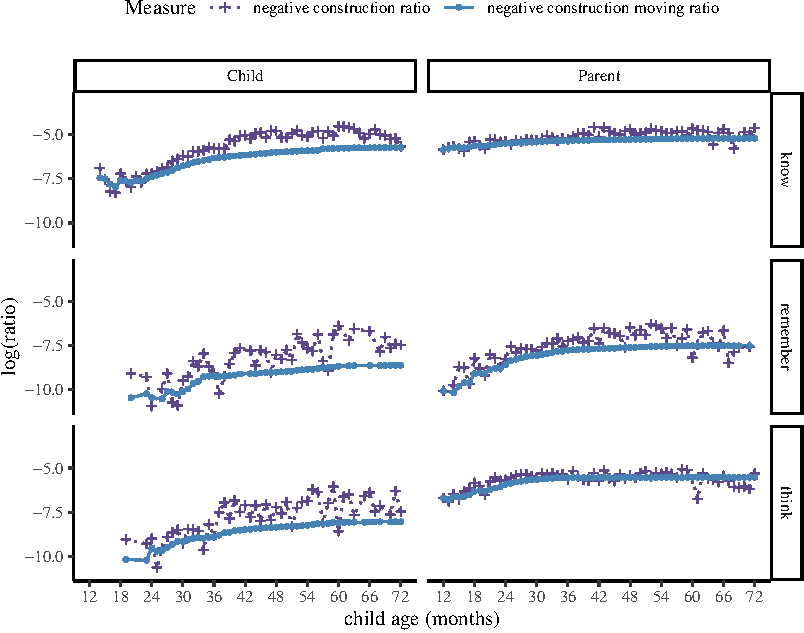
\includegraphics{figs/epistemic-1} \end{center}

\end{CodeChunk}
\caption[This image spans both columns]{Epistemic negation.}\label{fig:epistemic}
\end{figure*}

\begin{figure*}[h!]

\begin{CodeChunk}


\begin{center}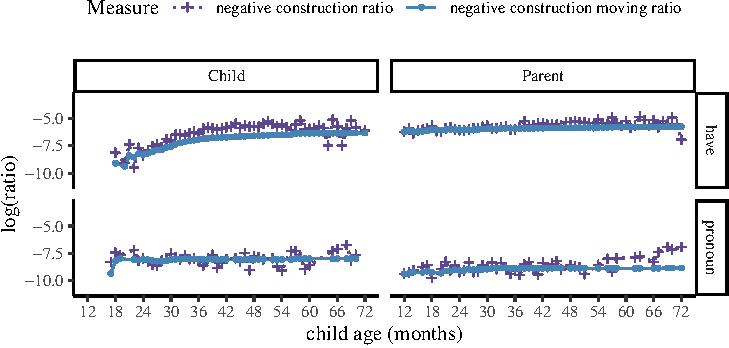
\includegraphics{figs/possession-1} \end{center}

\end{CodeChunk}
\caption[This image spans both columns]{Possession.}\label{fig:possession}
\end{figure*}

\begin{figure*}[h!]

\begin{CodeChunk}


\begin{center}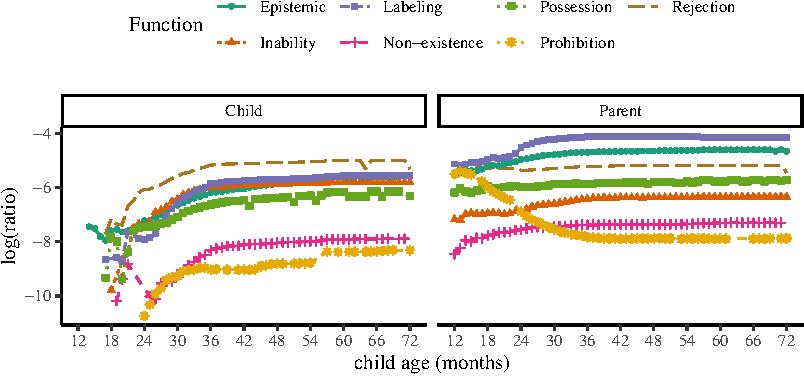
\includegraphics{figs/all-1} \end{center}

\end{CodeChunk}

\caption[This image spans both columns]{All functions; ratio measures plotted here are moving ratios.}\label{fig:all}
\end{figure*}

Based on the data analyzed here (Figure 6), comparing the developmental
trajectories of labeling with the three head verbs in child speech, the
production of negative utterances headed by \emph{know} are becoming
more regular at an earlier age (17-18 months) compared to that of
\emph{remember} (\textasciitilde19 months) or \emph{think}
(\textasciitilde20 months). Overall the production moving ratio of
utterances with \emph{know} is comparatively the highest.

\hypertarget{possession}{%
\subsubsection{Possession}\label{possession}}

The last function that we explored includes negative utterances that
denote possession. Specifically, we selected cases where the negative
morphemes are combined with auxiliary verbs to modify a head verb with
the lemma form \emph{have} (e.g.~(15)). We also included instances that
are individual noun phrases, where the heads of the noun phrases are
possessive pronouns modified by negative morphemes (e.g.~(16)).
Therefore cases in which the syntactic head of the negative morphemes is
a predicate of a copula verb (e.g.~``this is not mine'') were excluded
to separate from the function of labeling. The number of negative
utterances that were subjected to analysis for this function is 8,187
(child: 2,331; parent: 5,856).

~ (15) \emph{I don't have it}

~ (16) \emph{not mine}

Given Figure 7, the developmental trajectory for possession in child
speech appears to have notable differences depending on what the
negative morphemes are modifying. When their syntactic head is
\emph{have}, the pattern is comparable to the functions such as
rejection and labeling, where children are increasing their combination
of negative morphemes from 18 to 36 months. However, the production
moving ratio for utterances headed by possessive pronouns seems to be
relatively stable across different ages of the children.

\hypertarget{discussion}{%
\section{Discussion}\label{discussion}}

Using automatic annotations of large-scale corpora of child-parent
interactions, we presented production trajectories for seven negative
constructions that tend to express rejection, non-existence,
prohibition, inability, labeling, epistemic states, and possession
(Table 1). The results suggest that the production of almost all these
negative constructions (except for prohibition) emerges and gradually
increases within the 18-36 months age range (Figure 8). Their production
frequencies remain stable and regular after 36 months and relatively
close to parents' levels of production.

It is important to note that similar to prior studies, our conclusions
are limited to negation in children's production. While it is possible
that patterns in children's production reflect their comprehension and
semantic development overall, this is not guaranteed. Systematic
experiments testing children's comprehension of negative utterances with
different communicative functions are also necessary to better
understand the origins and developmental trajectory of negation.

For future work, we would like to explore several directions. First, one
limitation of our work here is that to more thoroughly examine and
potentially model the developmental trajectories of child production,
certain production-specific factors (e.g.~length of utterance, ease of
pronunciation) should be taken into account as well. In addition, we aim
to investigate the production trajectory of positive counterparts to our
negative structures (e.g.~``I know'' for ``I don't know''). Comparisons
of negative utterances in relation to their positive counterparts would
allow us to further analyze the developmental paths of negation within
specific constructions.

To validate the findings here at a closer angle, we also intend to
examine negative utterances produced by individual children with our
methods and analyses. Lastly, our experiments thus far have concentrated
on larger syntactic structures at the utterance level, hence cases where
negation is used as discourse markers to respond to previous
utterance(s) were excluded. However, these instances also have important
semantic and conceptual roles in the communication between children and
parents (e.g.~Parent: \emph{do you want some bread?}; Child: \emph{no no
no}). Thus inclusions of negative structures at a more comprehensive
level would be able to paint a more clear picture about the development
of negation.

\hypertarget{references}{%
\section{References}\label{references}}

\setlength{\parindent}{-0.1in} 
\setlength{\leftskip}{0.125in}

\noindent

\hypertarget{refs}{}
\leavevmode\hypertarget{ref-diaparser}{}%
Attardi, G., Sartiano, D., \& Yu, Z. (n.d.). DiaParser attentive
dependency parser. \emph{Submitted for Publication}.

\leavevmode\hypertarget{ref-bloom1970language}{}%
Bloom, L. M. (1970). \emph{Language development: Form and function in
emerging grammars} (PhD thesis). Columbia University.

\leavevmode\hypertarget{ref-cameron2007part}{}%
Cameron-Faulkner, T., Lieven, E., \& Theakston, A. (2007). What part of
no do children not understand? A usage-based account of multiword
negation. \emph{Journal of Child Language}, \emph{34}(2), 251.

\leavevmode\hypertarget{ref-choi1988semantic}{}%
Choi, S. (1988). The semantic development of negation: A
cross-linguistic longitudinal study. \emph{Journal of Child Language},
\emph{15}(3), 517--531.

\leavevmode\hypertarget{ref-clark2010adult}{}%
Clark, E. V. (2010). Adult offer, word-class, and child uptake in early
lexical acquisition. \emph{First Language}, \emph{30}(3-4), 250--269.

\leavevmode\hypertarget{ref-darwin1872expression}{}%
Darwin, C. (1872). \emph{The expression of the emotions in man and
animals}. John Murray.

\leavevmode\hypertarget{ref-demuth2006word}{}%
Demuth, K., Culbertson, J., \& Alter, J. (2006). Word-minimality,
epenthesis and coda licensing in the early acquisition of English.
\emph{Language and Speech}, \emph{49}(2), 137--173.

\leavevmode\hypertarget{ref-macwhinney2000childes}{}%
MacWhinney, B. (2000). \emph{The childes project: Tools for analyzing
talk. Transcription format and programs} (Vol. 1). Psychology Press.

\leavevmode\hypertarget{ref-nordmeyer2018individual}{}%
Nordmeyer, A., \& Frank, M. C. (2018). Individual variation in
children's early production of negation. In \emph{CogSci}.

\leavevmode\hypertarget{ref-pea1978}{}%
Pea, R. (1978). \emph{The development of negation in early child
language} (PhD thesis). University of Oxford.

\leavevmode\hypertarget{ref-sagae2010morphosyntactic}{}%
Sagae, K., Davis, E., Lavie, A., MacWhinney, B., \& Wintner, S. (2010).
Morphosyntactic annotation of childes transcripts. \emph{Journal of
Child Language}, \emph{37}(3), 705--729.

\leavevmode\hypertarget{ref-sanchez2019childes}{}%
Sanchez, A., Meylan, S. C., Braginsky, M., MacDonald, K. E., Yurovsky,
D., \& Frank, M. C. (2019). Childes-db: A flexible and reproducible
interface to the child language data exchange system. \emph{Behavior
Research Methods}, \emph{51}(4), 1928--1941.

\leavevmode\hypertarget{ref-dg}{}%
Tesnière, L. (1959). \emph{Éléments de syntaxe structurale}. Paris:
Klincksieck.

\leavevmode\hypertarget{ref-de1979form}{}%
Villiers, P. A. de, \& Villiers, J. G. de. (1979). Form and function in
the development of sentence negation. \emph{Papers and Reports on Child
Language Development}, \emph{17}, 57--64.

\leavevmode\hypertarget{ref-wei2006time}{}%
Wei, W. W. (2006). Time series analysis. In \emph{The oxford handbook of
quantitative methods in psychology: Vol. 2}.

\bibliographystyle{apacite}


\end{document}
